% ████████████████████████████████████████████████████████████████████████████████
%
%   CODEX ΔΦ — HL-IMAGENET RCC / PHASE 2 DIAGNOSTIC LENS
%   SOFTWARE ARCHITECTURE (HL-RCCA-DL v1.0)
%   ────────────────────────────────────────────────────────────────────────────
%   CANONICAL ATTRIBUTION-PRESERVING SOFTWARE ARCHITECTURE FOR ADDING A
%   DIAGNOSTIC / EVIDENCE LENS TO HL-IMAGENET AFTER RCC CONTEXT INJECTION AND
%   UPSTREAM PHASE 2 CLASSIFIER EVOLUTION WITHOUT CLAIMING AUTHORSHIP OF THE
%   ORIGINAL CLASSIFIER, WITHOUT CHANGING CLASSIFIER RUNTIME BEHAVIOR, WITHOUT
%   PROMOTING PHASE 2 RESULTS INTO FINAL BENCHMARK CLAIMS, AND WITHOUT CLAIMING
%   THAT RCC IMPROVED CLASSIFIER ACCURACY
%
%   VERSION
%   ───────
%   v1.0 — Diagnostic Lens Genesis Layer · Locked ·
%          RCC / AEFL Context Boundary, Upstream Phase 2 Attribution Boundary,
%          Phase 2 Evidence Surface Mapping, Attractor / Victim Diagnostics,
%          Confusion Gravity Wells, Feature-Reuse Warning Surface, Claim-Lock
%          Preservation, Non-Runtime Diagnostic Tooling, Architecture Delta,
%          and Future Phase 2.3 Governance
%
%   AUTHOR
%   ──────
%   James Paul Jackson
%   X / Twitter: @unifiedenergy11
%
%   SOURCE / AUTHOR ATTRIBUTION
%   ───────────────────────────
%   This document is a Codex-format software architecture and diagnostic
%   governance layer derived from the current public HL-ImageNet repository
%   state after:
%
%       • the original HL-ImageNet heuristic-learning image-classification
%         repository and experiment by the original/upstream author;
%
%       • James Paul Jackson's RCC / AEFL documentation-context injection,
%         which added root AI / RCC guidance, folder-level mini READMEs,
%         claim-boundary locks, local invariants, and safer AI/human navigation;
%
%       • the upstream Phase 2 classifier evolution, including a 10-class Tiny
%         ImageNet phase, phase2_signatures.py, hierarchy.py, soft scoring,
%         split-aware logging, and Phase 2 evaluation reports.
%
%   ATTRIBUTION BOUNDARY
%   ────────────────────
%   Original/upstream author contribution:
%
%       HL-ImageNet classifier concept, Phase 1 experiment, Phase 2 classifier
%       implementation, enriched Phase 2 representation space, hierarchy.py,
%       phase2_signatures.py, evaluation logs, and classifier behavior.
%
%   James Paul Jackson contribution so far:
%
%       RCC / AEFL repository context layer only:
%       root AI/RCC operating contract, folder-specific mini READMEs,
%       navigation surfaces, invariants, hooks, artifacts, examples, and
%       claim-boundary preservation.
%
%   Proposed contribution authorized by this document:
%
%       Diagnostic/evidence tooling only. No classifier behavior change.
%
%   SHORT REPO NAME
%   ───────────────
%       hl-imagenet
%
%   DIAGNOSTIC MODULE NAME
%   ──────────────────────
%       phase2_diagnostic_lens
%
%   DATE
%   ────
%   May 2026
%
%   STATUS
%   ──────
%   CANONICAL v1.0 SOFTWARE ARCHITECTURE LAYER —
%   NOT CLASSIFIER AUTHORSHIP · NOT PHASE 2 AUTHORSHIP · NOT RUNTIME BEHAVIOR
%   CHANGE · NOT CLASSIFIER IMPROVEMENT · NOT ACCURACY IMPROVEMENT · NOT A
%   CLAIM THAT RCC IMPROVED MODEL PERFORMANCE · NOT A STANDARD IMAGENET
%   BENCHMARK CLAIM · NOT A FINAL GENERALIZATION CLAIM · NOT A REPLACEMENT FOR
%   TRAIN/VALIDATION/TEST DISCIPLINE · NOT A CLAIM THAT DIAGNOSTICS PROVE
%   CORRECTNESS
%
%   PURPOSE
%   ───────
%   Define the complete software architecture for adding a Phase 2 diagnostic
%   lens to HL-ImageNet:
%
%       Phase 2 eval log
%       → confusion matrix parse
%       → per-class precision / recall
%       → victim score
%       → attractor score
%       → confusion gravity wells
%       → feature-reuse warnings
%       → recommendations
%       → JSON diagnostic artifact
%       → Markdown diagnostic report
%       → bounded next-step guidance.
%
%   HL-RCCA-DL v1.0 answers:
%
%       • What changed after RCC and upstream Phase 2?
%       • Which contribution belongs to whom?
%       • What diagnostic layer can be safely added before classifier changes?
%       • How can Phase 2 failure geometry be made visible?
%       • How do we prevent diagnostics from becoming inflated performance
%         claims?
%
%   WHAT THIS IS
%   ────────────
%   • A canonical architecture delta document
%   • A diagnostic/evidence architecture for Phase 2 logs
%   • An attribution-preserving contribution boundary
%   • A non-runtime analysis layer
%   • A repo-maintenance governance layer
%   • A bridge from RCC navigation into evidence diagnostics
%   • A safe prerequisite before Phase 2.3 classifier modification
%
%   WHAT THIS IS NOT
%   ───────────────
%   • Not a classifier behavior change
%   • Not an implementation of Phase 2 classifier logic
%   • Not an accuracy improvement
%   • Not proof that symbolic heuristics generalize
%   • Not a claim that RCC improved classifier performance
%   • Not a replacement for held-out test evaluation
%   • Not a neural-network comparison
%   • Not permission to promote early Phase 2 logs into final benchmark claims
%
%   CORE SOFTWARE EXTRACTION
%   ────────────────────────
%   HL-RCCA-DL v1.0 extracts the software invariant:
%
%       A Phase 2 diagnostic lens converts existing evaluation logs into
%       bounded evidence artifacts that expose class-attractor imbalance,
%       victim classes, confusion gravity wells, top-3 rescue gaps, and
%       feature-reuse warning surfaces without changing classifier behavior.
%
%   First runnable target:
%
%       Analyze latest logs/phase2/eval_phase2*.json
%
%   First artifact set:
%
%       logs/phase2/diagnostics/latest_phase2_diagnostic.json
%       logs/phase2/diagnostics/latest_phase2_diagnostic.md
%
%   CANONICAL SOFTWARE LOCK (v1.0)
%   ─────────────────────────────
%   • Diagnostics may inspect logs; they may not change classifier behavior
%   • Diagnostics must preserve original/upstream author attribution
%   • Diagnostics must preserve James RCC attribution boundary
%   • Diagnostics must not claim accuracy improvement
%   • Diagnostics must not alter Phase 2 logs
%   • Diagnostics must emit non-claim locks
%   • Diagnostics must separate train, validation, test, and external results
%     when such tags are available
%   • Diagnostics must treat feature reuse as a warning surface until
%     sample-level/class-node attribution exists
%   • Diagnostics must guide inspection before Phase 2.3 scoring changes
%
%   RCC / AEFL CONTEXT LOCK
%   ───────────────────────
%   RCC turns the repository into a navigable context field. It does not
%   improve classifier accuracy by itself.
%
%   PHASE 2 ATTRIBUTION LOCK
%   ────────────────────────
%   Phase 2 classifier work belongs to the original/upstream author lineage.
%   Future James contributions begin only at diagnostic/evidence tooling unless
%   classifier code is explicitly changed later and attributed as such.
%
%   NON-CLAIM LOCK
%   ──────────────
%   Diagnostic output may identify failure geometry, not prove correctness.
%   Attractor and victim scores are analysis metrics, not benchmark results.
%
%   AI PROMPT TRACEABILITY
%   ──────────────────────
%   Use this document as the canonical HL-ImageNet RCC / Phase 2 Diagnostic
%   Lens v1.0 software architecture. Build only diagnostic tooling until this
%   layer has emitted evidence artifacts and been reviewed. Do not change
%   classifier behavior in the same step.
%
%   SHADOW HEADER ALIGNMENT SEAL
%   ───────────────────────────
%   Preserve header discipline across future HL-RCCA-DL versions except for
%   explicitly additive refinements that improve attribution clarity,
%   diagnostic correctness, evidence artifacts, split discipline, README/RCC
%   surfaces, or safety-boundary clarity.
%
% ████████████████████████████████████████████████████████████████████████████████

\documentclass[12pt]{article}

\usepackage[margin=1in]{geometry}
\usepackage{amsmath,amssymb,amsfonts,amsthm}
\usepackage{booktabs,longtable,array}
\usepackage{hyperref}
\usepackage{listings}
\usepackage{xcolor}
\usepackage{tikz}
\usetikzlibrary{arrows.meta,positioning,shapes.geometric,fit,calc}

\newtheorem{axiom}{Axiom}
\newtheorem{definition}{Definition}
\newtheorem{proposition}{Proposition}
\newtheorem{requirement}{Requirement}
\newtheorem{remark}{Remark}
\newtheorem{corollary}{Corollary}

\lstset{
  basicstyle=\ttfamily\small,
  breaklines=true,
  columns=fullflexible,
  frame=single
}

\title{\textbf{Codex $\Delta\Phi$ — HL-ImageNet RCC / Phase 2 Diagnostic Lens (HL-RCCA-DL v1.0)}\\
\large Architecture Delta, Attribution Boundary, Attractor Diagnostics, Victim Scores, Confusion Gravity Wells, and Evidence Governance}
\author{\textbf{James Paul Jackson}\\[4pt]
\small Codex-format diagnostic architecture for HL-ImageNet repository evolution\\
\small \texttt{@unifiedenergy11}}
\date{May 2026}

\begin{document}
\maketitle

\begin{abstract}
HL-RCCA-DL v1.0 defines an attribution-preserving diagnostic architecture for
HL-ImageNet after RCC context injection and upstream Phase 2 classifier
evolution. The architecture adds no classifier behavior and claims no accuracy
improvement. Its purpose is to convert existing Phase 2 evaluation logs into
bounded diagnostic artifacts: per-class precision and recall, false-positive
attractor scores, false-negative victim scores, confusion gravity wells, top-3
rescue gaps, feature-reuse warnings, and recommendations for future inspection.
This document preserves the boundary between the original/upstream classifier
work and James Paul Jackson's RCC / AEFL repository-context contribution. It
locks the next valid step: build the diagnostic lens before attempting Phase
2.3 classifier changes.
\end{abstract}

%──────────────────────────────────────────────────────────────────────────────
\section{Core-Invariant Extraction Block}
%──────────────────────────────────────────────────────────────────────────────

The shortest faithful extraction of HL-RCCA-DL v1.0 is:

\[
\boxed{
\begin{array}{c}
\text{HL-RCCA-DL converts Phase 2 evaluation logs into diagnostic evidence}\\
\text{about attractors, victims, confusion gravity wells, and claim-safe}\\
\text{next steps without modifying classifier behavior.}
\end{array}
}
\]

The operative chain is:

\[
\boxed{
EvalLog
\rightarrow
ConfusionMatrix
\rightarrow
Precision/Recall
\rightarrow
AttractorScore
\rightarrow
VictimScore
\rightarrow
GravityWells
\rightarrow
Warnings
\rightarrow
Recommendations
\rightarrow
DiagnosticReport.
}
\]

\begin{remark}
The architecture is intentionally diagnostic-first. It does not authorize new
features, new scorer weights, or new performance claims.
\end{remark}

%──────────────────────────────────────────────────────────────────────────────
\section{Repository State and Delta}
%──────────────────────────────────────────────────────────────────────────────

The current repository state is:

\[
\boxed{
HL
=
HL_{original}
+
RCC_{James}
+
Phase2_{upstream}.
}
\]

where:

\[
HL_{original}
=
\text{Phase 1 symbolic heuristic-learning image-classification system},
\]

\[
RCC_{James}
=
\text{documentation-context and AI-navigation layer},
\]

\[
Phase2_{upstream}
=
\text{10-class Phase 2 classifier and evidence-log evolution}.
\]

\begin{definition}[RCC / AEFL Context Layer]
The RCC / AEFL context layer is a repository-navigation layer composed of a
root AI/RCC operating contract and folder-level mini READMEs. It makes folder
purpose, hooks, artifacts, invariants, and examples visible to humans and AI
agents.
\end{definition}

\begin{definition}[Phase 2 Diagnostic Lens]
A Phase 2 Diagnostic Lens is a non-runtime analysis layer that reads existing
evaluation artifacts and emits evidence summaries describing classifier failure
geometry.
\end{definition}

%──────────────────────────────────────────────────────────────────────────────
\section{Attribution Boundary}
%──────────────────────────────────────────────────────────────────────────────

\subsection{Original / Upstream Author Work}

The original/upstream author lineage owns:

\begin{itemize}
\item the HL-ImageNet classifier concept,
\item Phase 1 symbolic image classifier implementation,
\item sensors, scene graph, features, classifier, proof, evaluation, and logs,
\item Phase 2 classifier implementation,
\item \texttt{hlinet/classifier/hierarchy.py},
\item \texttt{hlinet/features/compounds/phase2\_signatures.py},
\item Phase 2 soft scoring and class signatures,
\item Phase 2 evaluation artifacts.
\end{itemize}

\subsection{James Paul Jackson Work}

James Paul Jackson owns the RCC / AEFL context contribution:

\begin{itemize}
\item root AI/RCC operating contract,
\item folder-specific mini READMEs,
\item local context beacons,
\item claim-boundary locks,
\item edit-boundary guidance,
\item agentic navigation framing.
\end{itemize}

\subsection{Authorized Next Contribution}

This document authorizes:

\begin{itemize}
\item diagnostic tooling,
\item architecture documentation,
\item log-derived reports,
\item no classifier behavior change.
\end{itemize}

\begin{axiom}[Attribution Preservation]
No diagnostic architecture may blur the boundary between upstream classifier
work and James's RCC / diagnostic contribution.
\end{axiom}

%──────────────────────────────────────────────────────────────────────────────
\section{Current Phase 2 Runtime Architecture}
%──────────────────────────────────────────────────────────────────────────────

The current runtime path is:

\[
\boxed{
Image
\rightarrow
SceneGraph
\rightarrow
Sensors
\rightarrow
Features
\rightarrow
Phase2Signatures
\rightarrow
Hierarchy
\rightarrow
Scorer
\rightarrow
Prediction
\rightarrow
EvalMetrics
\rightarrow
Phase2Logs.
}
\]

Expanded file path:

\begin{lstlisting}
data/phase2/<split>/<class_name>/
  -> hlinet/eval/dataset.py
  -> hlinet/eval/runner.py
  -> hlinet/classifier/predict.py
  -> hlinet/scene/builder.py
  -> hlinet/features/compounds/phase2_signatures.py
  -> hlinet/classifier/hierarchy.py
  -> hlinet/classifier/scorer.py
  -> hlinet/eval/metrics.py
  -> logs/phase2/eval_phase2_*.json
\end{lstlisting}

\begin{remark}
The diagnostic lens reads the final logs. It does not enter the prediction path.
\end{remark}

%──────────────────────────────────────────────────────────────────────────────
\section{Diagnostic Object Model}
%──────────────────────────────────────────────────────────────────────────────

Let \(C\) be the set of classes and \(M\) be the confusion matrix where:

\[
M_{ij}
=
\text{number of samples with true class } i
\text{ predicted as class } j.
\]

For class \(k\):

\[
TP_k = M_{kk},
\]

\[
FN_k = \sum_j M_{kj} - M_{kk},
\]

\[
FP_k = \sum_i M_{ik} - M_{kk}.
\]

Recall:

\[
Recall_k
=
\frac{TP_k}{TP_k + FN_k}.
\]

Precision:

\[
Precision_k
=
\frac{TP_k}{TP_k + FP_k}.
\]

Victim score:

\[
Victim_k
=
\frac{FN_k}{TP_k + FN_k}.
\]

Attractor score:

\[
Attractor_k
=
\frac{FP_k}{TP_k + FP_k}.
\]

\begin{definition}[Confusion Gravity Well]
A confusion gravity well is an off-diagonal pair \(i \rightarrow j\) with high
count \(M_{ij}\). It identifies a repeated collapse path where true class \(i\)
is absorbed by predicted class \(j\).
\end{definition}

\begin{axiom}[Failure Geometry Before Feature Surgery]
A classifier should not receive new hand-authored features until its dominant
confusion gravity wells, attractors, and victims are identified.
\end{axiom}

%──────────────────────────────────────────────────────────────────────────────
\section{Software Architecture}
%──────────────────────────────────────────────────────────────────────────────

The valid diagnostic implementation adds:

\begin{lstlisting}
docs/
  architecture/
    hl_imagenet_rcc_phase2_diagnostic_lens_v1_0.tex

hlinet/
  eval/
    diagnostics.py

scripts/
  run_phase2_diagnostics.py

logs/
  phase2/
    diagnostics/
      README.md
      .gitkeep
      latest_phase2_diagnostic.json
      latest_phase2_diagnostic.md
\end{lstlisting}

No valid implementation may modify:

\begin{lstlisting}
hlinet/classifier/predict.py
hlinet/classifier/scorer.py
hlinet/classifier/hierarchy.py
hlinet/features/compounds/phase2_signatures.py
\end{lstlisting}

during the same architecture-locked diagnostic pass.

\begin{requirement}[Input Contract]
The diagnostic tool must accept a Phase 2 JSON report path or default to the
latest \texttt{logs/phase2/eval\_phase2*.json} file.
\end{requirement}

\begin{requirement}[Output Contract]
The diagnostic tool must emit both JSON and Markdown artifacts.
\end{requirement}

\begin{requirement}[Non-Claim Contract]
Every diagnostic report must state that it does not prove correctness and does
not change classifier behavior.
\end{requirement}

%──────────────────────────────────────────────────────────────────────────────
\section{Validation Surface}
%──────────────────────────────────────────────────────────────────────────────

HL-RCCA-DL v1.0 is valid if:

\begin{enumerate}
\item architecture document exists,
\item diagnostics module imports,
\item script runs from repository root,
\item latest Phase 2 report is discovered,
\item JSON diagnostic artifact is emitted,
\item Markdown diagnostic artifact is emitted,
\item per-class precision and recall are computed,
\item attractor and victim scores are computed,
\item top confusion gravity wells are listed,
\item feature-reuse warnings are emitted when appropriate,
\item non-claim locks appear in output,
\item no classifier files are modified.
\end{enumerate}

Compact condition:

\[
\boxed{
ValidDL
\Longleftrightarrow
Docs
\wedge
Import
\wedge
Run
\wedge
Logs
\wedge
Metrics
\wedge
Reports
\wedge
Locks
\wedge
\neg RuntimeChange.
}
\]

%──────────────────────────────────────────────────────────────────────────────
\section{Falsification Surface}
%──────────────────────────────────────────────────────────────────────────────

HL-RCCA-DL v1.0 is weakened or invalid if:

\begin{itemize}
\item it changes classifier behavior,
\item it claims classifier improvement,
\item it claims RCC improved accuracy,
\item it edits historical logs,
\item it overwrites Phase 2 reports without preserving provenance,
\item it merges train, validation, and test metrics without labels,
\item it treats diagnostics as benchmark proof,
\item it hides attribution boundaries,
\item it omits non-claim locks,
\item or it recommends feature changes without showing failure geometry.
\end{itemize}

Compact invalidation rule:

\[
\left[
Diagnostic = RuntimeChange
\right]
\vee
\left[
Diagnostic = AccuracyClaim
\right]
\vee
\left[
RCC = ClassifierImprovement
\right]
\vee
\left[
NoAttributionBoundary
\right]
\Rightarrow
\text{invalid HL-RCCA-DL use}.
\]

%──────────────────────────────────────────────────────────────────────────────
\section{System Diagram}
%──────────────────────────────────────────────────────────────────────────────

\begin{center}
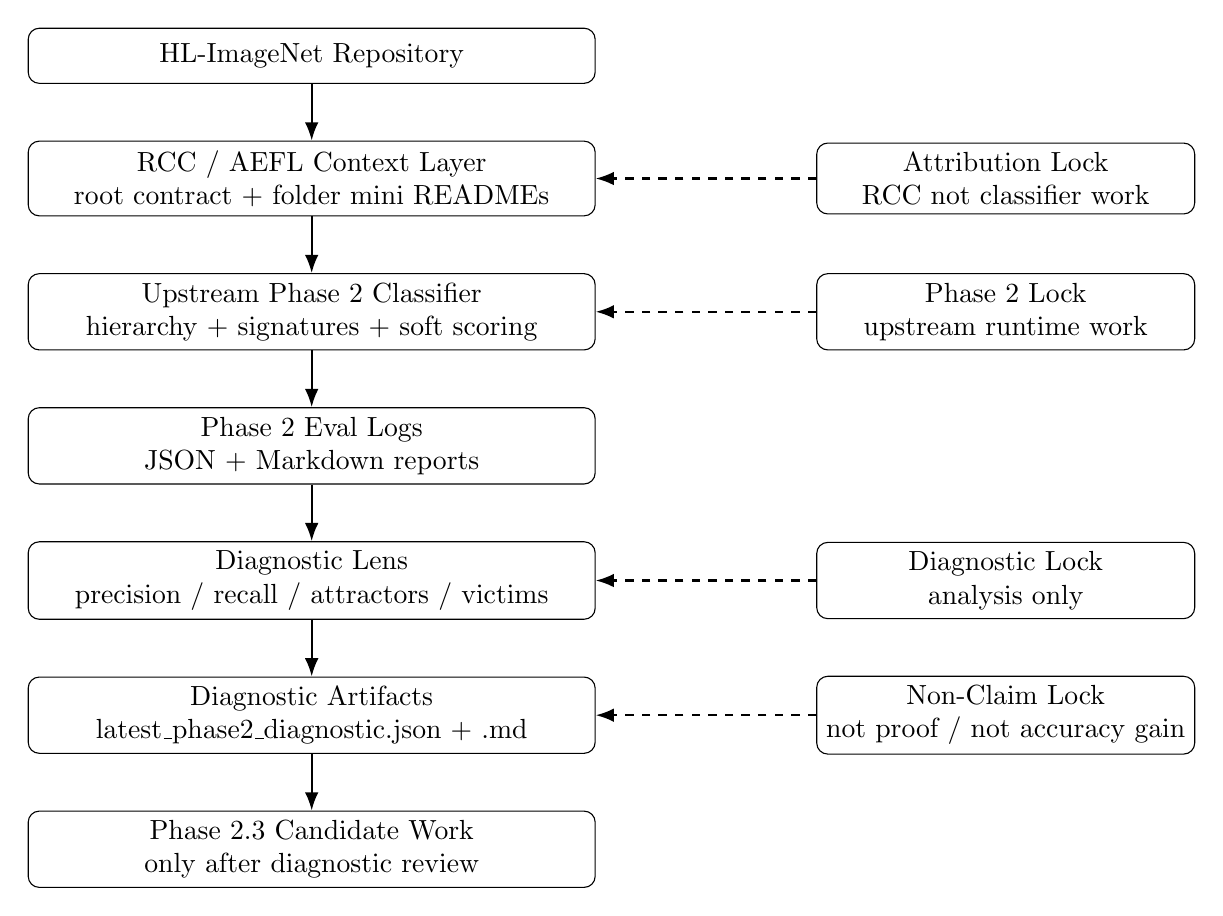
\begin{tikzpicture}[
  node distance=0.72cm,
  box/.style={rectangle, rounded corners, draw, align=center, minimum width=7.2cm, minimum height=0.70cm},
  smallbox/.style={rectangle, rounded corners, draw, align=center, minimum width=4.8cm, minimum height=0.62cm},
  arrow/.style={-Latex, thick}
]

\node[box] (repo) {HL-ImageNet Repository};
\node[box, below=of repo] (rcc) {RCC / AEFL Context Layer\\root contract + folder mini READMEs};
\node[box, below=of rcc] (phase2) {Upstream Phase 2 Classifier\\hierarchy + signatures + soft scoring};
\node[box, below=of phase2] (logs) {Phase 2 Eval Logs\\JSON + Markdown reports};
\node[box, below=of logs] (diag) {Diagnostic Lens\\precision / recall / attractors / victims};
\node[box, below=of diag] (report) {Diagnostic Artifacts\\latest\_phase2\_diagnostic.json + .md};
\node[box, below=of report] (next) {Phase 2.3 Candidate Work\\only after diagnostic review};

\draw[arrow] (repo) -- (rcc);
\draw[arrow] (rcc) -- (phase2);
\draw[arrow] (phase2) -- (logs);
\draw[arrow] (logs) -- (diag);
\draw[arrow] (diag) -- (report);
\draw[arrow] (report) -- (next);

\node[smallbox, right=2.8cm of rcc] (alock) {Attribution Lock\\RCC not classifier work};
\draw[arrow, dashed] (alock) -- (rcc);

\node[smallbox, right=2.8cm of phase2] (plock) {Phase 2 Lock\\upstream runtime work};
\draw[arrow, dashed] (plock) -- (phase2);

\node[smallbox, right=2.8cm of diag] (dlock) {Diagnostic Lock\\analysis only};
\draw[arrow, dashed] (dlock) -- (diag);

\node[smallbox, right=2.8cm of report] (nlock) {Non-Claim Lock\\not proof / not accuracy gain};
\draw[arrow, dashed] (nlock) -- (report);

\end{tikzpicture}
\end{center}

%──────────────────────────────────────────────────────────────────────────────
\section{Release Roadmap}
%──────────────────────────────────────────────────────────────────────────────

\subsection{v1.0 — Architecture Lock}

\begin{itemize}
\item this LaTeX document,
\item attribution boundary,
\item diagnostic definitions,
\item validation/falsification surfaces.
\end{itemize}

\subsection{v1.1 — Diagnostic Implementation}

\begin{itemize}
\item \texttt{hlinet/eval/diagnostics.py},
\item \texttt{scripts/run\_phase2\_diagnostics.py},
\item diagnostic JSON output,
\item diagnostic Markdown output.
\end{itemize}

\subsection{v1.2 — Sample-Level Attribution}

\begin{itemize}
\item sample-level prediction traces,
\item per-class feature activation distributions,
\item class-node attribution,
\item corrected feature-reuse reporting.
\end{itemize}

\subsection{v1.3 — Phase 2.3 Candidate Scoring Work}

\begin{itemize}
\item only after diagnostics,
\item attractor-balanced scoring,
\item class calibration,
\item no README performance promotion without test evidence.
\end{itemize}

%──────────────────────────────────────────────────────────────────────────────
\section{Public Framing}
%──────────────────────────────────────────────────────────────────────────────

Safe public framing:

\[
\boxed{
\text{I added an RCC repository-context layer and am proposing a diagnostic}
\atop
\text{lens to make Phase 2 classifier behavior easier to audit before}
\atop
\text{any future code changes.}
}
\]

Unsafe public framing:

\[
\boxed{
\text{I improved the classifier or implemented Phase 2.}
}
\]

That statement is not authorized by this document.

%──────────────────────────────────────────────────────────────────────────────
\section{Concluding Compression}
%──────────────────────────────────────────────────────────────────────────────

HL-ImageNet now contains three layers:

\[
\boxed{
OriginalClassifier
+
RCCContext
+
UpstreamPhase2.
}
\]

The next safe layer is:

\[
\boxed{
DiagnosticLens.
}
\]

The diagnostic law is:

\[
\boxed{
\text{Do not change the classifier until the failure geometry is visible.}
}
\]

The attribution law is:

\[
\boxed{
\text{Do not claim the upstream classifier as your own.}
}
\]

The RCC law is:

\[
\boxed{
\text{Context improves navigability; it does not imply accuracy gain.}
}
\]

The evidence law is:

\[
\boxed{
\text{Logs become useful when transformed into bounded diagnostic artifacts.}
}
\]

Thus HL-RCCA-DL v1.0 locks the correct next bridge: after RCC and upstream
Phase 2, the valid next contribution is diagnostic tooling. Build the lens.
Expose the attractors. Identify the victims. Preserve attribution. Then decide
whether Phase 2.3 should touch classifier behavior.

\end{document}
